%%%%%%%%%%%%%%%%%%%%%%%%%%%%%%%%%%%%%%%%%%%%%%%%%%%%%%%%%%%%%%%%%%%%%%
%%                           INTRODUCTION
%%%%%%%%%%%%%%%%%%%%%%%%%%%%%%%%%%%%%%%%%%%%%%%%%%%%%%%%%%%%%%%%%%%%%


\pagestyle{plain} % No headers, just page numbers
\pagenumbering{arabic} % Arabic numerals
\setcounter{page}{1}


\chapter{Introduction}
The rapid internet adoption in everyday life and the workplace has presented us with new security challenges. Users are more active on the internet, giving attackers more opportunities to attack unsuspecting victims. There are various technical security measures such as firewall, encryption, threat hunting software, and engaging automation to mitigate these challenges. However, studies have shown that the human layer is the weakest link in the security chain \cite{jampen} and attackers usually start by targeting the most vulnerable link before performing other detrimental attacks. These attacks with human interaction are generally known as "Social Engineering Attacks." Prevalent social engineering attacks such as phishing, pretexting, baiting, quid pro quo, and tailgating use psychological manipulation to trick users into making security mistakes or giving away sensitive information. This thesis will cover strategies to help people understand phishing and different detection techniques through our role-playing gameplay.

\section{What is phishing?}
Phishing is one of the most prevalent social engineering attacks in which attackers target users by contacting them through email, telephone, or text message by attackers posing as a legitimate entity \cite{phishing, apwg}. Unfortunately, these attacks are challenging to detect as attackers use the computing infrastructure to fool the victim into doing something but are doing something else while the computing system is working as intended. Due to this, even users with a high-end security system can be victims. An example of such is the infamous case of John Podesta \cite{Podesta}, Hilary Clinton's campaign chairman for the 2016 presidential election. The "googlemail.com" in the domain successfully tricked John Podesta and the Clinton campaign's computer help desk to trust the email (See fig:\ref{fig:Podesta}).

Phishing attacks are constantly evolving with different tricks. For example, although Podesta's email shows it was initially generated from "googlemail.com," that might not be true. There are different spoofing techniques attackers can use to hide the sender's identity. Another common trick attackers use (also present in Podesta's email) is hiding the link behind some text or button. The displayed text might not be the destination of the links. Failure to pay attention to such details can have massive consequences.

\begin{figure}[ht]
    \centering
    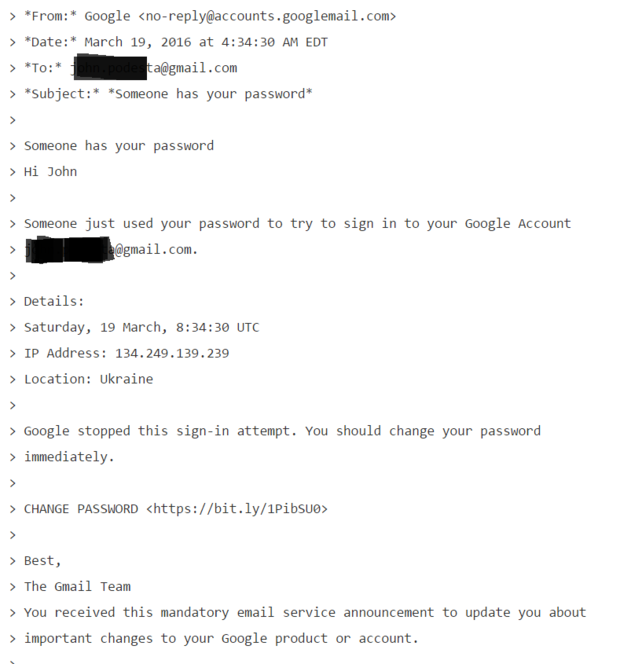
\includegraphics[scale=0.7]{{./podesta.png}}
    \caption[Phishing email sent to John Podesta]{Phishing email sent to John Podesta}
    \label{fig:Podesta}
\end{figure}

Successful phishing attacks are very costly to organizations. In 2020, phishing attacks cost US businesses more than \$1.8 billion, up from \$1.7 billion in 2019 \cite{vade}. In addition, these attacks can also lead to credential/account compromise leading to leaks of sensitive information. In 2014, an attack was successful on an invasion of celebrity iCloud accounts, leading to the embarrassing leaking of nude photos. The leak was initially considered due to a breach on Apple services, but it was later a phishing attack pretending to be Apple and Google and asking them to change their password \cite{duke_2014, guardian_2014}.

Phishing attacks are continuously rising and have doubled since early 2020. In July 2021 alone, APWG saw 260,642 phishing attacks \cite{apwg}. Additionally, Proofpoint found that more than 75\% of organizations faced phishing attacks in 2021 \cite{proofpoint}. These uprising trends in attacks have shown some serious need for mitigations for phishing attacks.

\section{Current Mitigations}
The prevention of phishing attacks can be divided into three steps \cite{vayansky}. The first step to stop a phishing attack is preventing the attack from reaching the end-user. We have seen multiple studies on phishing prevention with the help of the machine learning approach \cite{yang_zheng_wu_wu_wang_2021, sahingoz_buber_demir_diri_2019}. Although these models may catch some sites, it is impossible to filter out and prevent phishing attacks. The phisher can easily make a new site and learn to create better contextual attacks, preventing these models from being fully effective.

It is impossible to stop all the attacks as attackers usually design their attacks to reach vulnerable users. However, many web browsers and email clients are already prepared to warn users of any suspicious activities they detect. For example, browsers use active warnings such as "This page is not secure warnings" to warn the users of any certificates they fail to verify or pop up windows with a sign that the site they are on is suspected of forgery. In addition, there are other passive indicators, such as different shades of link highlights in the address bar, security lock signs, etc., that browsers use. Active warnings prevent more attacks \cite{vayansky}, but attackers can easily bypass these warnings by creating new sites and new contextual websites.

\begin{figure}[h]
    \centering
    
\includegraphics[scale=0.7]{{./browser_cues.png}}
    \caption[Browser cues on links]{Browsers uses different shades to indicate the primary link and the secondary links.}
    \label{fig:browser_cues}
\end{figure}

The final step to avoid phishing emails is user training. A study done by Proofpoint shows that 34\% of US respondents believe emails with familiar logos are safe \cite{proofpoint}. The study indicates a general lack of awareness about phishing campaigns among the general population. There are many tools used for phishing training. One of the most common tools to train users is cyber security videos. However, a study shows that these videos are only efficient only if the user pays attention through all of them \cite{what_hack}. We can also find other techniques such as reading materials and cyber security classes to raise awareness among users.

Although these training help users recognize phishing attacks, simply knowing does not provide helpful strategies for identifying phishing attacks. In addition, the lack of contextual information in these videos leaves room for improvement. Therefore, an interactive user program that conveys the information with a better approach is necessary. Our approach to using the game to spread awareness tries to tackle this problem.

\section{Litearature Review}
The gaming approach in education endeavors is not novel and has been used for over a decade \cite{almeida_2012}. There have been arguments for gaming in education. Prensky \cite{prensky} in "Digital game-based learning" shows that playing "action" video and computer games has a positive impact on enhancing students' visual selective attention. He further argues that video games are the best opportunity to engage kids in real learning. This argument was further studied by Almeida \cite{almeida_2012} and verified that when games are used against the control group, significant increases in factual knowledge occur.

Several studies have used different gaming approaches to train phishing campaigns again. Hendrix et al. \cite{hendrix_al_sherbaz_bloom_2016} investigated whether games can be effective cyber security training tools with some of the popular games designed for cyber security training. Their study indicated positive signs, although there was insufficient evidence to draw definite conclusions. We will look at some popular work below, separated by category.

\subsection{Board and card games}
There have been some studies based on non-computer-based games. For example, Control-Alt-Hack \cite{control_alt_hack} tries to educate the user with the help of a card game. Similarly, "Smells Phishy?" is another non-computer-based game that tries to raise awareness about online phishing scams. Both these game depends on cards to divide the task and learn skills. Although both the games had shown promise in their approach, non-computer-based games have some inherent limitations. The games require pre-setup (with the need for the cards and boards) and make it harder to use than computer-based games. Furthermore, the current approaches only teach users about phishing attacks. The limited skills these games provide may not be best suited as an individual training module.

\subsection{Phishing Link training}
There have been numerous computer games about phishing. One common category many studies focus on is training users to verify phishing links. Anti-Phishing Phil \cite{anti_phishing_phil} is one of the pioneers in this field. Their gameplay puts the user as a fish. The goal of the fish is to grow larger by eating the good bugs (non-phishing links). Phish Phinder \cite{phish_phinder} is another example of link based training game that has similar gameplay and story to Anti-Phishing Phil but builds upon the game with more levels and interaction. Baral et al. \cite{gamified_appraoch} has a similar concept with a balloon shooting game. The goal of these games is to differentiate the phishing links and actual links. However, these games do not consider the context of the email. Attackers use psychological manipulation such as creating a sense of urgency, fake giveaways or making it seem like an email from somebody you know to trick people into clicking these links.

\subsection{Role playing game}
"What.Hack" \cite{what_hack} saw the shortcomings of the link-based game and developed gameplay that train the user on links as well as email context. "What.Hack" puts the user as a player required to process emails to acquire contracts and protect their network from cybercriminals. It approaches the training by having the user role play as a victim and look at different techniques that could be found in actual attacks.

The contextual emails addressed one of the most significant shortcomings of link-based games. The game successfully educated users with similar concepts as link-based games and added context to the links. The result from "What.Hack" clearly shows users' preference for their gameplay compared to Anti-Phishing Phil. Moreover, the game demonstrated significant improvement compared to other games in detecting phishing emails \cite{what_hack}.

\section{Objective}
"What.Hack" clearly demonstrated that role-playing games with contextual emails were more effective than existing gameplays. Unfortunately, we could not find any other significant study that tried to build upon this finding. Therefore, we have developed gameplay inspired by "What.Hack" but approached the role-playing aspect as an attacker instead of a victim.

General phishing training such as videos and reading materials has taught users what to look for as victims. However, we believe looking at the attacker's perspective will help users understand what the attacker might look for while creating a phishing email. This will also help complement the currently available training games.

Our goals for the study can be summarized as:

\begin{itemize}
    \setlength\itemsep{-0.6em}
    \item Develop a role-playing game to train the users about phishing through an attackers perspective
    \item Compare our results with the existing study
\end{itemize}
